% This document should be printed double-sided on standard A4 paper
% The default options for memoir are:
%   letterpaper,10pt,twoside,onecolumn,openright,final
\documentclass[a4paper,11pt]{memoir}

% Remove the 'draft' option when you're ready to submit
% It will remove the line numbers, and the "Draft generated on..." line on
% the title page
\usepackage[draft]{packages}

\author{Alex Pearce}
% Use texorpdfstring to stop TeX strings being mangled in PDF viewer toolbars
\title{%
  Measurements of charm production and \texorpdfstring{\CP\ }{CP} violation at \lhcb
}
\date{July 2016}

% Fill in the PDF metadata
% Don't need to specify the title as we passed the pdfusetitle option to 
% hyperref
\hypersetup{%
  pdfauthor={\theauthor},
  pdfcreator={\theauthor}
}

\begin{document}

% Title page
\begin{titlingpage}
  \begin{center}
    \textbf{\huge\thetitle}

    \vspace{0.5cm}

    \textbf{\Large\theauthor}

    \vfill

    A thesis submitted to The University of Manchester\\
    for the degree of Doctor of Philosophy\\

    \vspace{0.8cm}

    Particle Physics Group\\
    School of Physics and Astronomy\\
    Faculty of Engineering and Physical Sciences\\
    \textbf{\thedate}

    \vspace{0.8cm}

    
\includegraphics[width=0.4\textwidth]{university_logo}

    \iftoggle{draft}{%
      \vspace{0.8cm}
      \texttt{Draft generated on \today}
    }{}
  \end{center}
\end{titlingpage}

\frontmatter

\chapter{Abstract}

\lipsum[1-2]


\cleardoublepage

\chapter{Summary for the layperson}


\cleardoublepage

\tableofcontents

\mainmatter
\iftoggle{draft}{\linenumbers}{}

\part{%
  Charm production at
  \texorpdfstring{%
    $\sqrts = \SI{13}{\TeV}$
  }{%
    sqrt(s) = 13 TeV
  }
}

\chapter{Introduction}
\label{chap:prod:introduction}

This \lcnamecref{chap:prod} describes a measurement of charm and \ccbar\ 
production, performed using data taken at $\sqrts = \SI{13}{\TeV}$ with the 
\lhcb\ detector.
At the \ac{LHC}, a given charm hadron \PHc\ can either be produced in the 
proton-proton interaction or in the decays of \PB hadrons.
The latter mechanism is called secondary production, whilst the former is 
called prompt production.
The type of charm hadron produced can either be charmonium, such as the \PJpsi 
meson, or open charm, whose net charm quantum number is non-zero.
This measurement is concerned with the prompt production of open charm hadrons.
Charm hadrons originating from the strong decay of prompt excited charm states 
are also considered to be prompt, and here no attempt is made to distinguish 
between the two sources.

Measurements of \ccbar\ and \bbbar\ cross-sections at the \ac{LHC} are made to 
test the predictions of \ac{QCD}.
The production rate of heavy flavour hadrons is expected to vary as a function 
of hadron \pT\ and rapidity \rapidity, defined as
\begin{equation}
  y = \frac{1}{2}\ln{\frac{E + p_{z}}{E - p_{z}}},
  \label{eqn:prod:introduction:rapidity}
\end{equation}
and so experimental measurements can be compared with both the shape of 
theoretical predictions as a function of \pTy\ as well as to the total 
integrated rate.
Measurements can also be used as inputs to constrain predictions.
Heavy flavour production rates are also used to estimate sensitivities of 
experimental searches for rare decays, and also as inputs to atmospheric 
neutrino experiments, where charm production enters as a background process.

Measuring \ccbar\ and \bbbar\ cross-sections at \lhcb\ is complementary to such 
efforts made using the \acp{GPD}, due to the unique rapidity range of the 
detector, as well as its ability to cleanly reconstruct low \pT\ hadrons.

\section{Analysis overview}
\label{chap:prod:introduction:analysis_overview}

The measured cross-section for the inclusive production of an open charm hadron 
\PHc\ from proton-proton collisions can be expressed as
\begin{equation}
  \xsec(\PHc) = \frac{%
    N(\HcTof)
  }{%
    \eff(\HcTof)\cdot\bfrac(\HcTof)\cdot\intlumi
  },
  \label{eqn:prod:introduction:cross_section}
\end{equation}
where $N(\HcTof)$ is the number of reconstructed and selected prompt charm 
hadrons \PHc\ in some final state $f$; \eff\ is the efficiency of fully 
reconstructing and selecting the decay \HcTof, given that it was produced; 
\bfrac\ is the branching fraction of the decay; and \intlumi\ is the integrated 
luminosity.
To compare with the shapes of theoretical predictions, double differential 
cross-sections can be determined in bins of charm hadron \pT\ and \rapidity, 
using the width $\Delta\pT$ of the bin in \pT\ and the width $\Delta\rapidity$ 
of the bin in rapidity in which the yield and efficiency measurements were made
\begin{equation}
  % There is a "\left." here, which is invisible, to balance the "\right\rvert"
  \left.\frac{\dif^{2}{\xsec(\PHc)}}{\dif{\pT}\dif{\rapidity}}\right\rvert_{i}
    = \frac{1}{\Delta\pT\Delta\rapidity}
      \frac{%
        N_{i}(\HcTof)
      }{%
        \eff_{i}(\HcTof)\cdot\bfrac(\HcTof)\cdot\intlumi
      },
  \label{eqn:prod:introduction:differential_cross_section}
\end{equation}
where $i$ is the index of the \pTy\ bin.

The analysis presented in this \lcnamecref{chap:prod} measures the double 
differential cross-sections of \PDzero, \PDp, \PDsplus, and \PDstarp open charm 
mesons.\footnotemark\
The final states chosen are \DzToKpi, \DpToKpipi, \DspTophipi with \phiToKK, 
and \DstToDzpi with \DzToKpi, the branching fractions of which are listed in 
\cref{tab:prod:introduction:branching_ratios}.
Charge conjugation is implied, in that the cross-sections are measured as the 
combined rate of meson and anti-meson production.
The measurements are made in the \pT\ range \pTrange{0}{15} and the rapidity 
range \yrange{2}{4.5}.
In \rapidity, the measurements are made in five bins of width 0.5, and in \pT\ 
the bins are \SI{1}{\GeVc} in width in the regions \pTrange{0}{1} and 
\pTrange{4}{15}, and are \SI{0.5}{\GeVc} in width in the region \pTrange{1}{4}.

\footnotetext{%
  The excited \PD state is, formally, the \PDstp\ meson, but will be referred 
  to throughout as `\PDstarp'.
}

\begin{table}
  \centering
  \caption{%
      Branching ratios for the different decay 
      modes~\cite{PDG2014,Alexander:2008aa}.
      The \DspTophipi\ branching fraction includes the branching fraction of 
      \phiToKK\@.
  }
  \label{tab:prod:introduction:branching_ratios}
  \begin{tabular}{lS[table-format=1.2(2)]}
  \toprule
  Decay mode  & {\bfrac\ (\si{\percent})} \\
  \midrule
  \DzToKpi    & 3.88 \pm 0.05             \\
  \DpToKpipi  & 9.13 \pm 0.19             \\
  \DspTophipi & 2.24 \pm 0.13             \\
  \DstToDzpi  & 67.7 \pm 0.5              \\
  \bottomrule
\end{tabular}

\end{table}

From the double differential measurements, several derived quantities are 
computed, namely the ratio of charm production rates measured at $\sqrts = 
\SI{13}{\TeV}$ to those measured by \lhcb\ at 
\SI{7}{\TeV}~\cite{LHCb-PAPER-2012-041}, ratios of production rates between 
charm mesons, open charm hadron cross-sections integrated across the \pTy\ 
space, and integrated \ccbar\ cross-sections.
Each integrated per-meson cross-section is the sum over all \pTy\ bins of the 
respective double differential measurements.
The total \ccbar\ cross-sections can be computed using fragmentation fractions, 
each a measurement of the transition probability $f(\cToHc)$ that a charm quark 
will hadronise to a particular open charm hadron.
Given the fragmentation fraction and the integrated cross-section, the 
integrated \ccbar\ cross-section can be computed as
\begin{equation}
  \xsec{(\ccbar)} = \frac{\xsec(\PHc + \APHc)}{2f(\cToHc)}.
  \label{eqn:prod:introduction:ccbar_cross_section}
\end{equation}
The factor $\sfrac{1}{2}$ accounts for the inclusion of the charge conjugate 
(anti-charm) states in the measurement, which have been noted explicitly here 
to avoid ambiguity.
For this analysis, the fragmentation fractions are taken from the 
\ac{PDG}~\cite{PDG2008}, who compute them as averages of measurements made at 
\epem\ colliders operating at a centre-of-mass energy close to the 
\PUpsilonFourS resonance.
These values are given in \cref{tab:prod:introduction:fragmentation_fractions}, 
where the transition probability for \PDzero, $f(\decay{\Pcharm}{\PDzero})$, 
includes contributions from \DstToDzpi\ decays.

\begin{table}
  \caption[Charm hadron fragmentation fractions]{%
    Charm hadron fragmentation fractions~\cite{PDG2008}.
  }
  \label{tab:prod:introduction:fragmentation_fractions}
  \centering
  \begin{tabular}{cc}
  \toprule
  $\PHc$   & $f(\cToHc)$       \\
  \midrule
  \PDz     & $0.565 \pm 0.032$ \\
  \PDp     & $0.246 \pm 0.020$ \\
  \PDsplus & $0.224 \pm 0.028$ \\
  \PDstarp & $0.080 \pm 0.017$ \\
  \bottomrule
\end{tabular}

\end{table}

\subsection{Treatment of uncertainties}
\label{chap:prod:introduction:uncertainties}

Throughout the analysis, the method of \acl{MC} error propagation is used.
With this, each quantity entering 
\cref{eqn:prod:introduction:differential_cross_section} is assumed to be drawn 
from some \acf{PDF} with a known set of parameters, and then ten thousand 
numbers are sampled from that \ac{PDF}.
When performing operations using such quantities, the operations are performed 
on the sample vectors, and then statistics on the result can be computed on the 
new, resulting sample vector.
This technique is used as an analytical error analysis of the measurement is 
complex: what enters into the cross-section is the inverse of the efficiency, 
for example, the corresponding \acl{PDF} of which may not be obvious, in 
particular whether the uncertainties can be treated as Gaussian.
The use of \acl{MC} error propagation simplifies such analyses.

% Don't use pTyrange here as it causes a long, unbroken line
An example cross-section, measured in the region \pTrange{12}{13}, 
\yrange{2.5}{3}, is given in 
\cref{fig::prod:introduction:uncertainties:posterior}.
The blue curve shows the \ac{PDF} of the cross-section, as modelled by the 
\ac{MC} error propagation technique, when only the statistical uncertainty is 
considered, whilst the green curve also includes the contributions from the 
systematic uncertainties.
The green curve is not symmetric, and the mode is shifted with respect to that 
of the blue.

Unless stated otherwise, each quantity that is measured directly is assumed to 
follow a normal distribution, whose mean is equal to the measured value and 
whose width is equal to the measured uncertainty on that value.
The computation of that measured uncertainty will be described when the 
respective quantities are first discussed.
When the results of operations using such inputs are presented, such as 
cross-sections, the central value given is the most probable value of the 
sample vector representing the result, and the lower and upper uncertainty 
bounds are given by the \SI{15.9}{\percent} and \SI{84.1}{\percent} percentiles 
either side of the central value.

\begin{figure}
  \centering
  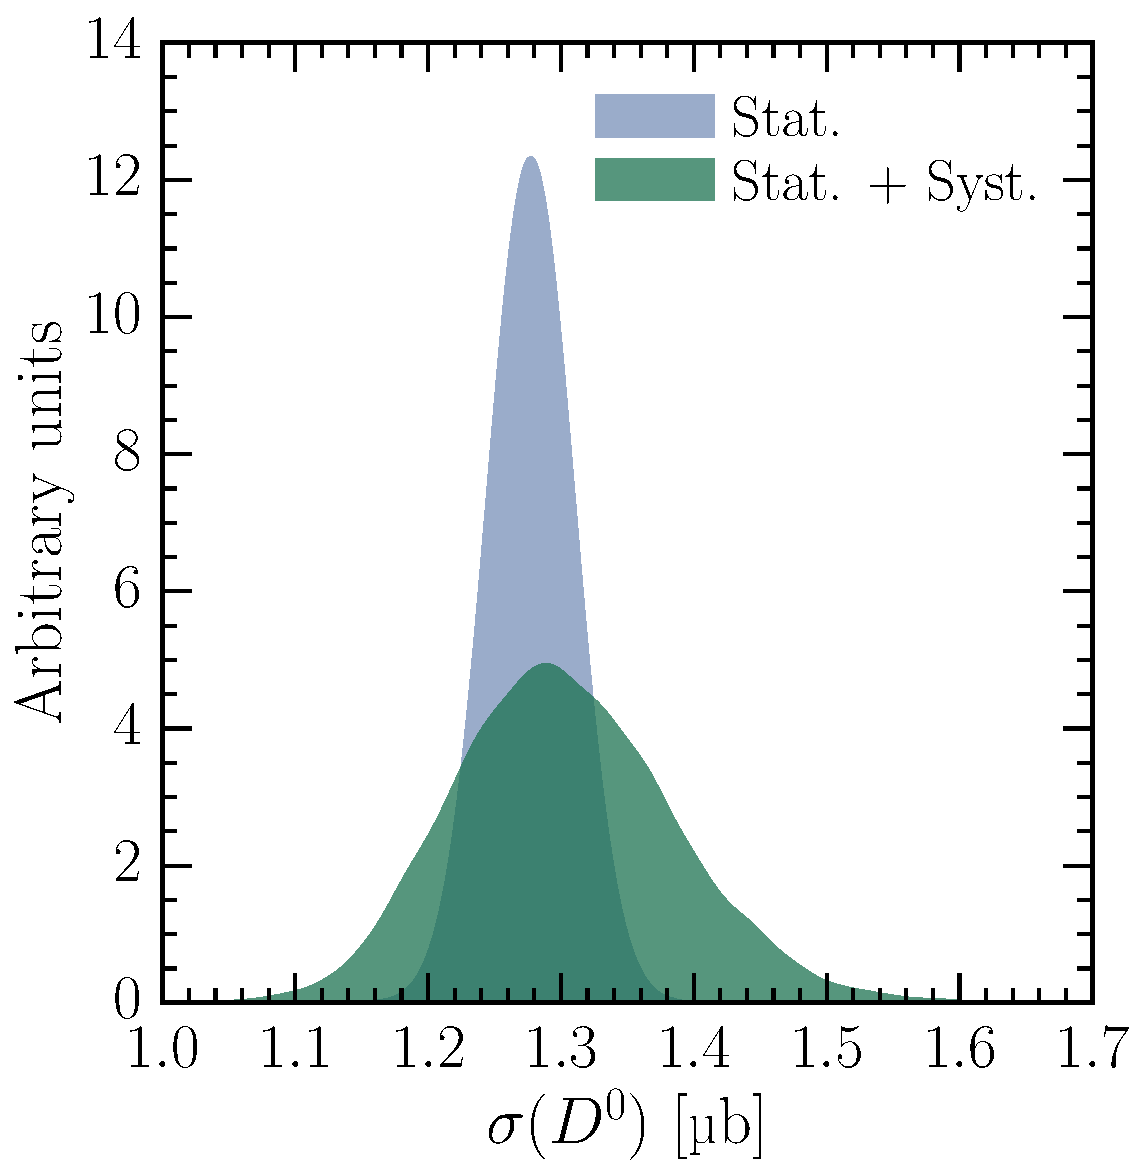
\includegraphics[width=\linewidth]{production/D0ToKpi_posterior_pdf}
  \caption{%
    Posterior probability densities for a measurement of the \PDzero 
    cross-section in the region \pTyrange{12}{13}{2.5}{3}.
    The blue curve shows the density including contributions only from the 
    statistical uncertainty on the prompt signal count.
    The green curve shows the density including contributions from all 
    uncertainties that enter the measurement.
  }
  \label{fig::prod:introduction:uncertainties:posterior}
\end{figure}

\subsection{Document structure}
\label{chap:prod:introduction:structure}

The data used for the measurements were collected in July 2016, under a set of 
special conditions used for the restart of the \ac{LHC} after \ac{LS1}.
The conditions of the \ac{LHC} and of the \lhcb\ detector during this period 
will be described in \cref{chap:prod:data}, along with a description of the 
corresponding simulated data and a summary of the integrated luminosity 
measurement.
The reconstruction and selection of the collected data will be presented in 
\cref{chap:prod:sel}.
The extraction of the prompt charm yields is made on the fully reconstructed 
and selected data using the method of maximum likelihood fits, as described in 
\cref{chap:prod:fitting}.
The evaluation of the associated efficiencies is performed using a mixture of 
simulated \acl{MC} data and dedicated calibration samples, and is discussed in 
\cref{chap:prod:effs}, after which the systematic uncertainties associated with 
all procedures used in the measurement are evaluated, for which the description 
and results are given in \cref{chap:prod:syst}.
Finally, the cross-sections themselves are computed, and are presented in 
\cref{chap:prod:results}.


\chapter{Theory and motivation}
\label{chap:prod:theory}

For an observable cross-section \xsec\ of inclusive production of some object 
$P$, $\decay{h_{A}h_{B}}{PX}$, involving two initial-state hadrons $h_{A}$ and 
$h_{B}$, the dominant contribution to a prediction can be expressed as the 
convolution of several terms
\begin{equation}
  \xsec = \sum_{a,b} \sigma_{a,b} \otimes f_{a,A} \otimes f_{b,B},
  \label{eqn:prod:theory:factorisation}
\end{equation}
where the sum runs over all parton types $a$ and $b$ in the respective hadrons 
$h_{A}$ and $h_{B}$; $\sigma_{a,b}$ is the cross-section of the hard partonic 
interaction $\decay{ab}{PX}$; and $f$ is the \ac{QCDPDF} for the interacting 
parton in the respective hadron~\cite{Collins:1989gx,Forte:2013wc}.
The parton-parton cross-sections $\sigma_{a,b}$, for processes such as heavy 
quark pair production via gluon-gluon fusion shown in 
\cref{fig:intro:lhcb:hf_production:gg_fusion}, can be computed using 
perturbative \ac{QCD}.
The computations of the \acp{QCDPDF} involve low-energy processes below the 
\ac{QCD} scale, and so must be evaluated using non-perturbative \ac{QCD} 
instead.
Clearly, the computation of any cross-section at the \ac{LHC} relies on being 
able to evaluate \cref{eqn:prod:theory:factorisation}, including the 
computation of production rates of the Higgs boson and particles beyond the 
\ac{SM}, and hence on a knowledge of the \acp{QCDPDF}.
As the \acp{PDF} cannot be computed from first principles, they must be derived 
be alternate means, and in practice are constrained using measurements of 
cross-sections by experiments.
Additional measurements of cross-sections can constrain the \acp{QCDPDF} 
further, improving their precision.

Parton density functions are parameterised in terms of \bjorkenx, the fraction 
of the total hadron momentum carried by the interacting parton, and 
\pdfqsquared, a measure of momentum transfer and inversely proportional to the 
spatial `scale' at which the hadron can be probed, with a larger \pdfqsquared\ 
corresponding to a finer resolvable structure.
The \ac{QCDPDF} $f(\bjorkenx, \pdfqsquared)$ for a particular hadron is an 
intrinsic property, and so, for example, experimental measurements that can 
constrain the \ac{QCDPDF} in high-energy proton collisions help not only the 
experiments at that collider, but also experiments at other proton colliders.
This is possible as the evolution of the \acp{QCDPDF} over \pdfqsquared\ for a 
given value of \bjorkenx\ is described by the \ac{DGLAP} differential 
equations~\cite{Gribov:1972ri,Dokshitzer:1977sg,Altarelli:1977zs}.
Measuring a wide range of \bjorkenx\ is important as the individual 
contributions to the total \ac{QCDPDF}, such as from the gluons and the valence 
quarks, vary strongly as a function of \bjorkenx, as shown in 
\cref{fig:prod:theory:pdf_sets}.
The usage of the \ac{DGLAP} equations requires an initial \ac{QCDPDF} from 
which to evolve to different scales, however, as the dependence on \bjorkenx\ 
cannot be computed perturbatively.
Such inputs were first provided by \ac{DIS} experiments, which probe the proton 
structure by colliding leptons and protons.
The subsequent evolution of the \acp{PDF} have been driven by additional 
experimental measurements, and by an improved theoretical understanding of the 
use of the perturbative expansion that must be employed when solving the 
\ac{DGLAP} equations.

The treatment of experimental inputs is a matter of debate, as there are 
somewhat arbitrary choices to be made on what experimental inputs should be 
used, and on how the various experimental uncertainties should be treated.
As a result, different groups of theorists provide so-called `\ac{QCDPDF} 
sets', which differ not only in the treatment of the inputs, but also in the 
treatment of the \emph{theoretical} uncertainties.
These include, for example, the choice of order to which the perturbation 
series are evaluated, and whether the value of the perturbation series scale is 
a parameter of the fit or if it is fixed.
For heavy flavour production, additional uncertainties arise from the choice of 
\emph{fragmentation function} models~\cite{Kneesch:2007ey}, which describe how 
the heavy quarks transition into the observed hadrons, a factor which is not 
included in the factorisation theorem shown in 
\cref{eqn:prod:theory:factorisation}.\footnotemark\
The different \ac{QCDPDF} sets can be used to compute different cross-section 
predictions, and so further experimental measurements can help to distinguish 
between predictions.

\footnotetext{%
  The fragmentation functions are generally assumed to be process independent, 
  e.g.\ they are the same for heavy flavour hadron production from \qqbar\ 
  production at both $\Pelectron\APelectron$ and $\Pproton\Pproton$ colliders.
  They cannot be computed perturbatively, and are extracted from experimental 
  measurements.
}

\begin{figure}
  \begin{subfigure}[b]{0.5\textwidth}
    \centering
    \begin{tikzpicture}
  \node[anchor=south west, inner sep=0] (image) at (0, 0) {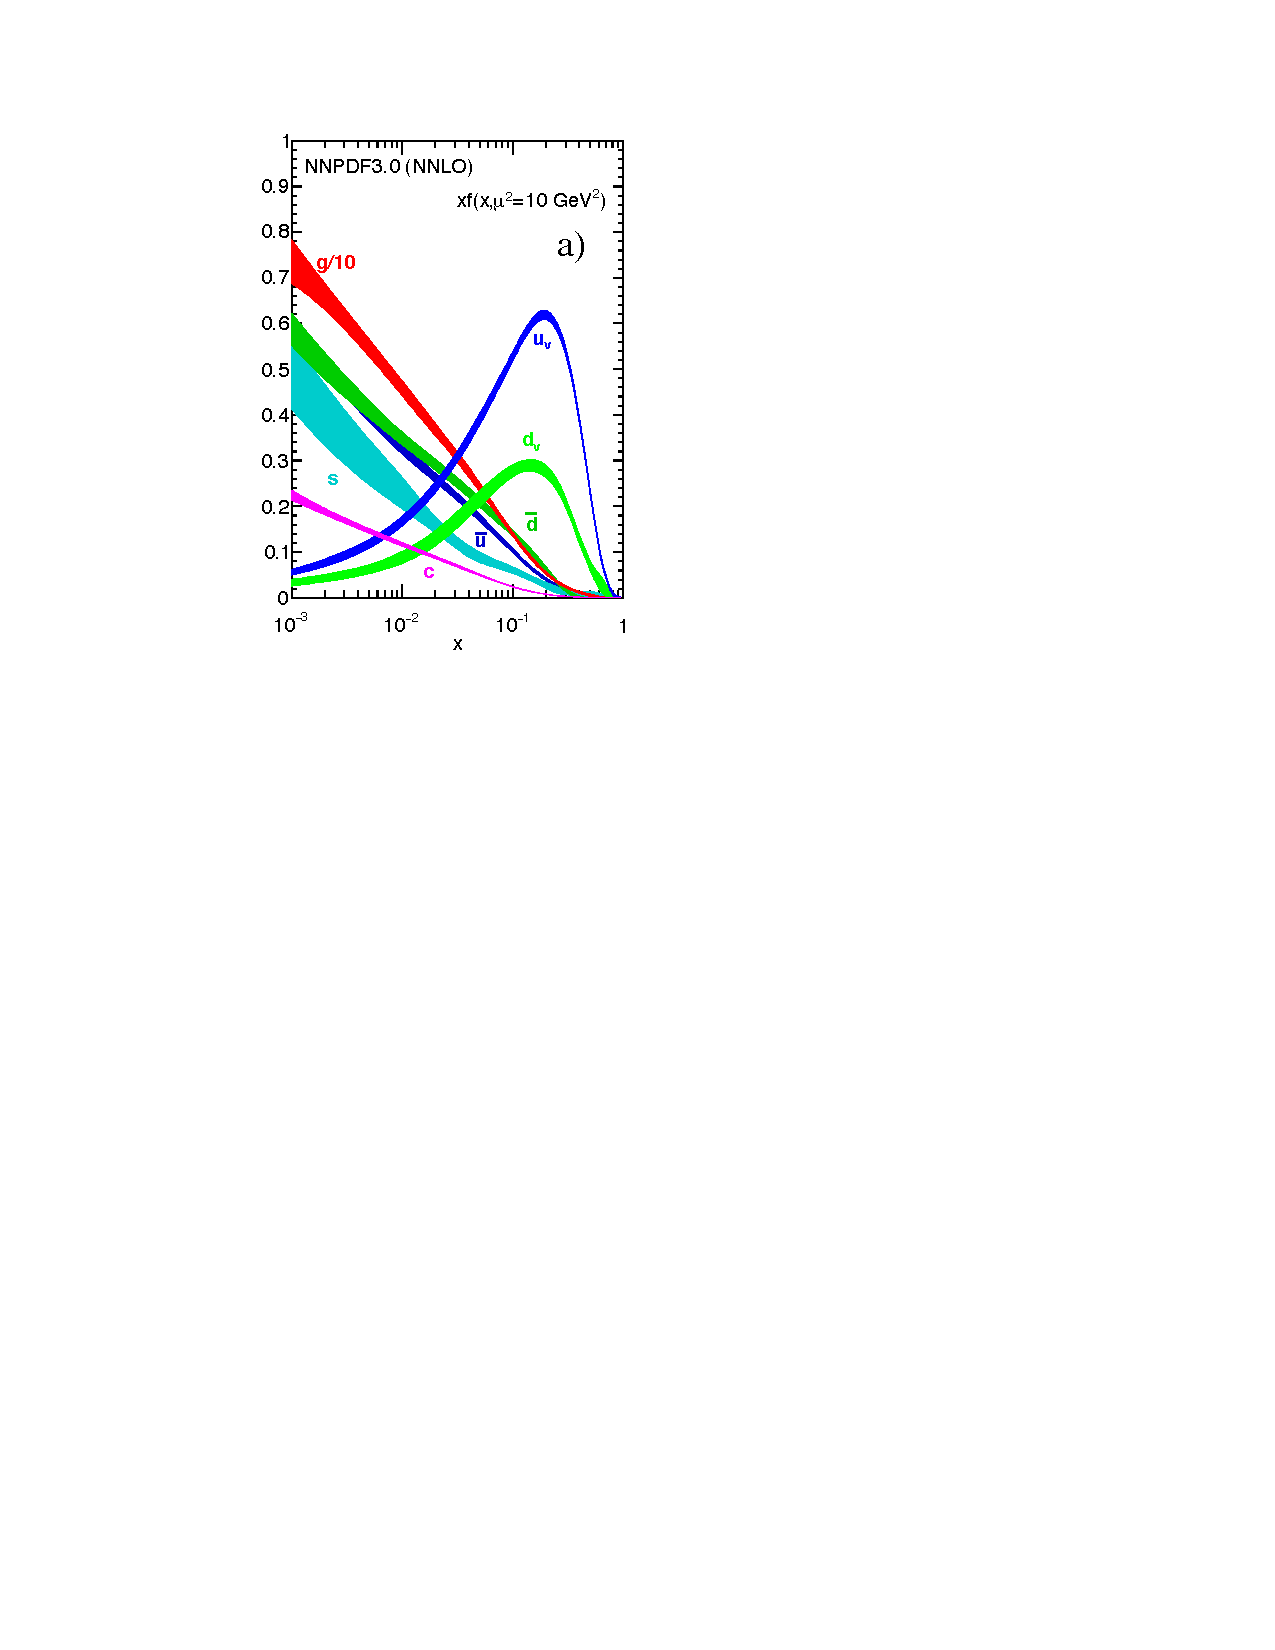
\includegraphics[width=\textwidth]{production/pdf_sets_low_qsquared}};
  \begin{scope}[x={(image.south east)}, y={(image.north west)}]
    % Grid to help find coordinates on the image
    % \draw[step=0.02, gray, very thin] (0, 0) grid (1, 1);
    % Box to cover 'a)' label
    \path[fill=white] (0.8, 0.74) rectangle (0.9, 0.82);
  \end{scope}
\end{tikzpicture}

    \caption{Low \pdfqsquared}
    \label{fig:prod:theory:pdf_sets:low_qsquared}
  \end{subfigure}
  \begin{subfigure}[b]{0.5\textwidth}
    \centering
    \begin{tikzpicture}
  \node[anchor=south west, inner sep=0] (image) at (0, 0) {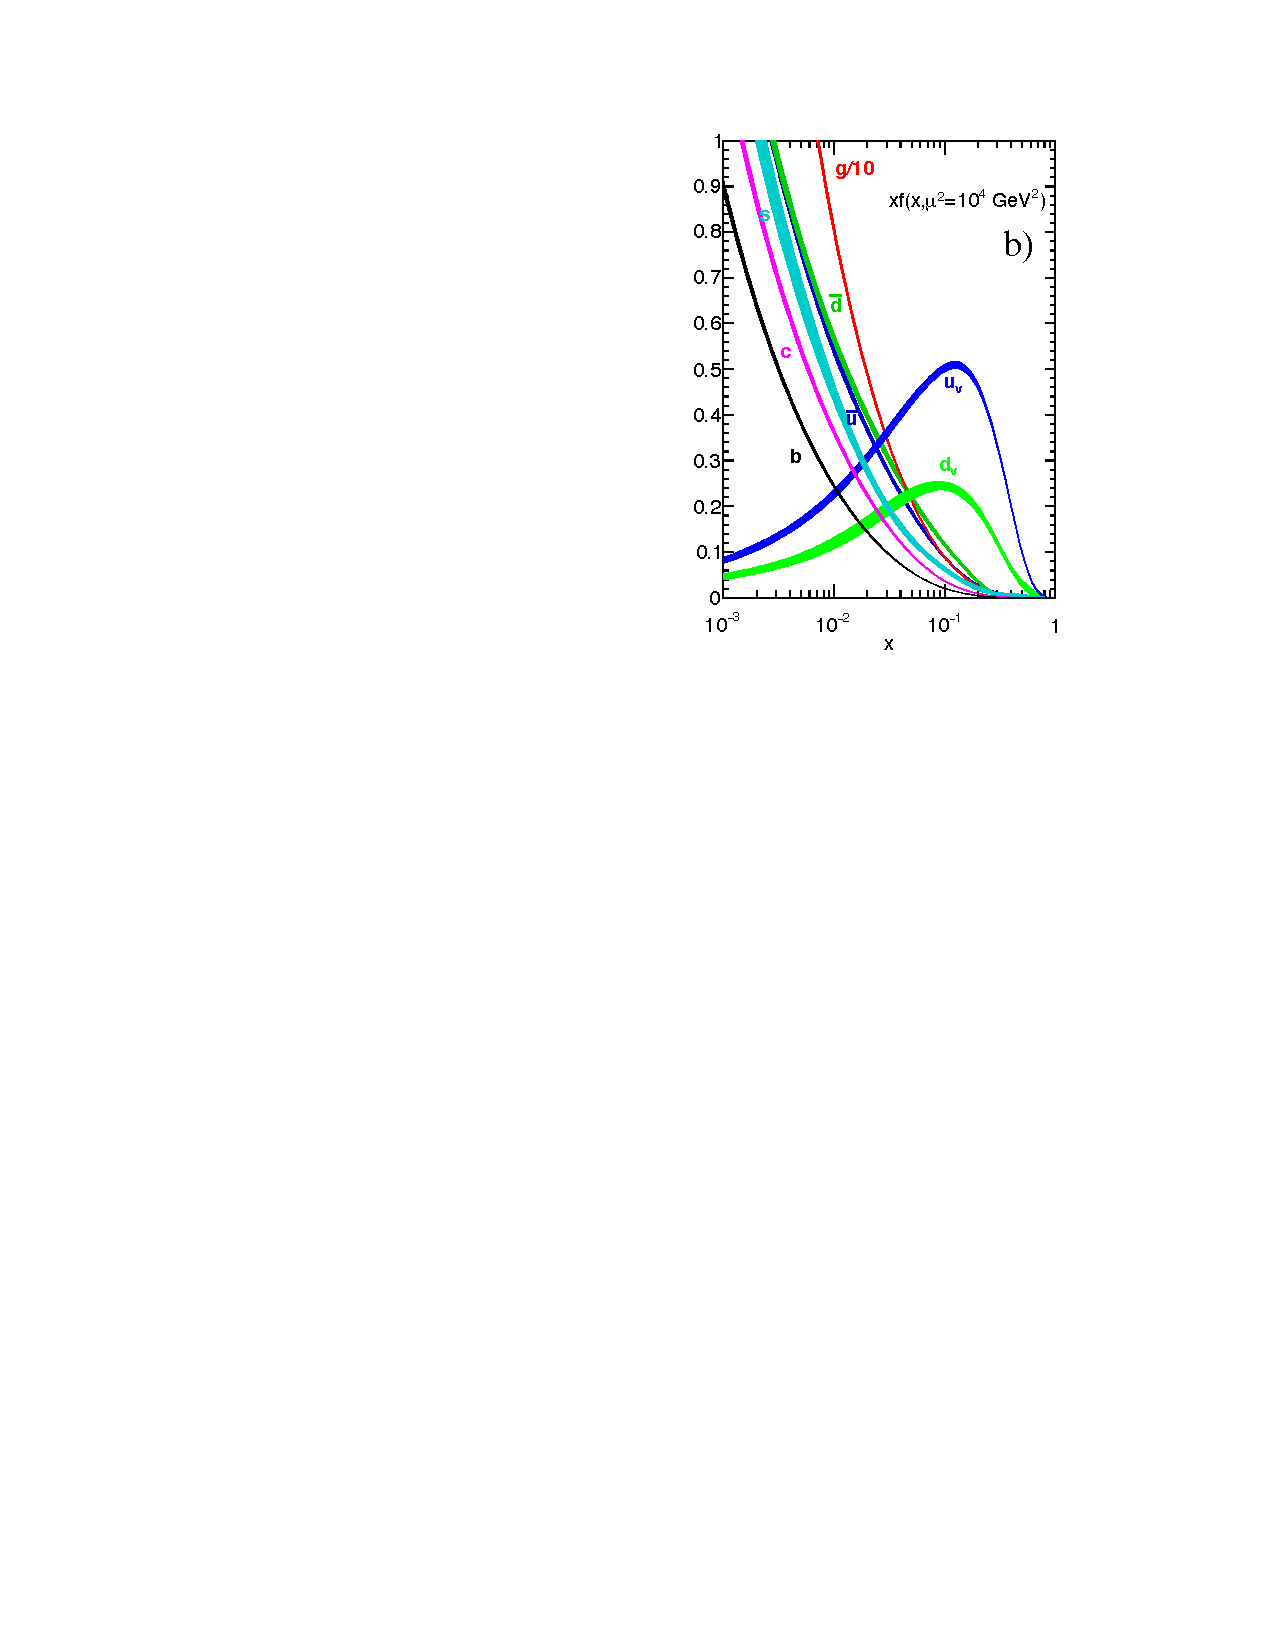
\includegraphics[width=\textwidth]{figures/production/pdf_sets_high_qsquared}};
  \begin{scope}[x={(image.south east)}, y={(image.north west)}]
    % Grid to help find coordinates on the image
    % \draw[step=0.02, gray, very thin] (0, 0) grid (1, 1);
    % Box to cover 'b)' label
    \path[fill=white] (0.82, 0.74) rectangle (0.94, 0.82);
  \end{scope}
\end{tikzpicture}

    \caption{High \pdfqsquared}
    \label{fig:prod:theory:pdf_sets:high_qsquared}
  \end{subfigure}
  \caption{%
    Sets of proton \aclp{QCDPDF} for low \pdfqsquared\ 
    (\subref*{fig:prod:theory:pdf_sets:low_qsquared}) and high \pdfqsquared\ 
    (\subref*{fig:prod:theory:pdf_sets:high_qsquared}), illustrating both 
    \bjorkenx\ and \pdfqsquared\ dependence~\cite{PDG2014}.
    Each band represents the \ac{QCDPDF} for a specific parton, as a function 
    of \bjorkenx, shown on the $x$-axis.
    The $\Pup_{\text{v}}$ and $\Pdown_{\text{v}}$ bands show the contributions 
    from the valance quarks, the \Pgluon band shows the gluon contribution, and 
    the other bands show the contribution from flavour-specific sea quarks.
  }
  \label{fig:prod:theory:pdf_sets}
\end{figure}

\subsection{Experimental input}
\label{chap:prod:theory:pdfs:inputs}

Today, inputs from both \ac{DIS} and hadron-hadron collider experiments serve 
to constrain proton \acp{QCDPDF} over a wide range of \bjorkenx\ and 
\pdfqsquared\ values.
The most recent and most powerful \ac{DIS} measurements have been made by the 
\hone\ and \zeus\ collaborations at the \hera\ $\Pe\Pproton$ 
collider~\cite{Abramowicz:1900rp}.
However, these measurements are largely constrained to measure values of 
\bjorkenx\ above \num{e-4}, leading to large uncertainties at low \bjorkenx.
This low-\bjorkenx\ region is particularly interesting to study not only 
because the current \ac{QCDPDF} uncertainties there are large, but also because 
it is where both the gluon and the sea quark contributions to the total 
\ac{QCDPDF} are large, as shown in \cref{fig:prod:theory:pdf_sets}, and so 
low-\bjorkenx\ measurements probe phenomenologically different processes.

In a hard \decay{2}{2} process, such as $\Pgluon\Pgluon$ fusion or \qqbar\ 
annihilation to a heavy quark pair, the extent in \bjorkenx\ that can be probe 
with heavy flavour hadron production measurements is given by
\begin{equation}
  {\bjorkenx}_{\text{min}} = e^{\pm\rapidity}\frac{%
    \sqrt{\pT^{2} + m_{\Pquark}^{2}}
  }{%
    \sqrts
  },
  \label{fig:prod:theory:hf_bjorkenx}
\end{equation}
where \rapidity\ and \pT\ parameterise the hadron kinematics, and $m_{q}$ is 
the mass of the heavy quark in the hadron under study~\cite{Zenaiev:2015rfa}.
There is then a wide range of \bjorkenx\ values that can be probed at proton 
colliders, with the highest sensitivity to low \bjorkenx\ provided by charm 
production measurements.\footnotemark\
At the \ac{LHC}, the dominant production mechanism is gluon-gluon fusion, as 
depicted in \cref{fig:intro:lhcb:hf_production:gg_fusion}, and so measurements 
at the \ac{LHC} are able to provide particularly strong constraints on the 
gluon densities.
Charm cross-sections have been measured in the $|\rapidity| < 0.5$ region for 
$\pT > \SI{1}{\GeVc}$ at \sqrtseq{2.76}\ and \sqrtseq{7}\ by the \alice\ 
collaboration~\cite{Abelev:2012sx,ALICE:2012ik,ALICE:2011aa},
and for pseudorapidity $|\Eta| < 2.1$ in the \pT\ region $3.5 < \pT < 
\SI{100}{\GeVc}$ at \sqrtseq{7} by the \atlas\ 
collaboration~\cite{Aad:2015zix}.

\footnotetext{%
  The charm quark mass is four times less than that of the bottom quark.
}

Measurements of charm production at \sqrtseq{7}\ were made by the \lhcb\ 
collaboration~\cite{LHCb-PAPER-2012-041}.
By \cref{fig:prod:theory:hf_bjorkenx}, measurements of charm hadron production 
for \pT\ values of the order of \SI{1}{\GeVc} at the lowest rapidities 
accessible to \lhcb\ can probe \bjorkenx\ values down to the order of \SI{e-6}, 
with lower values possible for measurements at a higher \sqrts, as shown in 
\cref{fig:prod:theory:prosa_x_regions}.
These measurements, along with similar measurements of beauty hadron production 
at \lhcb~\cite{LHCb-PAPER-2013-004} and the aforementioned \hone\ and \zeus\ 
measurements, have been used by the \prosa\ 
collaboration~\cite{Zenaiev:2015rfa} to constrain the proton \aclp{QCDPDF}, 
where they see a significant reduction on the gluon \ac{QCDPDF} uncertainty 
when including the \lhcb\ data, with respect to using the \hera\ data only, as 
shown in \cref{fig:prod:theory:prosa_gluon_pdf_fit}.
It is expected that additional measurements, at \sqrtseq{13}, can be used to 
further reduce the gluon \ac{QCDPDF} uncertainties~\cite{Gauld:2015yia}.

% \begin{figure}
%   \centering
%   \begin{tikzpicture}
  \begin{feynman}[scale=1.25,transform shape]
    \vertex (a);
    \vertex [right=of a] (b);

    \vertex [above left=of a] (i1) {\(\Pgluon\)};
    \vertex [below left=of a] (i2) {\(\Pgluon\)};

    \vertex [above right=of b] (f1) {\(\Pquark\)};
    \vertex [below right=of b] (f2) {\(\APquark\)};
    % Vertex in between b and f2, for the radiative gluon
    \vertex (bf1) at ($(b)!0.5!(f2)$);
    \vertex [right=of b] (f3);

    \diagram* [large] {
      (a) -- [gluon, edge label=\(\Pgluon\)] (b),
      (i1) -- [gluon] (a),
      (i2) -- [gluon] (a),
      (b) -- [fermion] (f1),
      (f2) -- [fermion] (b),
      (bf1) -- [gluon, edge label=\(\Pgluon\)] (f3),
    };
  \end{feynman}
\end{tikzpicture}

%   \caption{%
%     Feynman diagram of \qqbar\ pair production via \qqbar\ annihilation.
%   }
%   \label{fig:prod:theory:qqbar_annihilation}
% \end{figure}

\begin{figure}
  \centering
  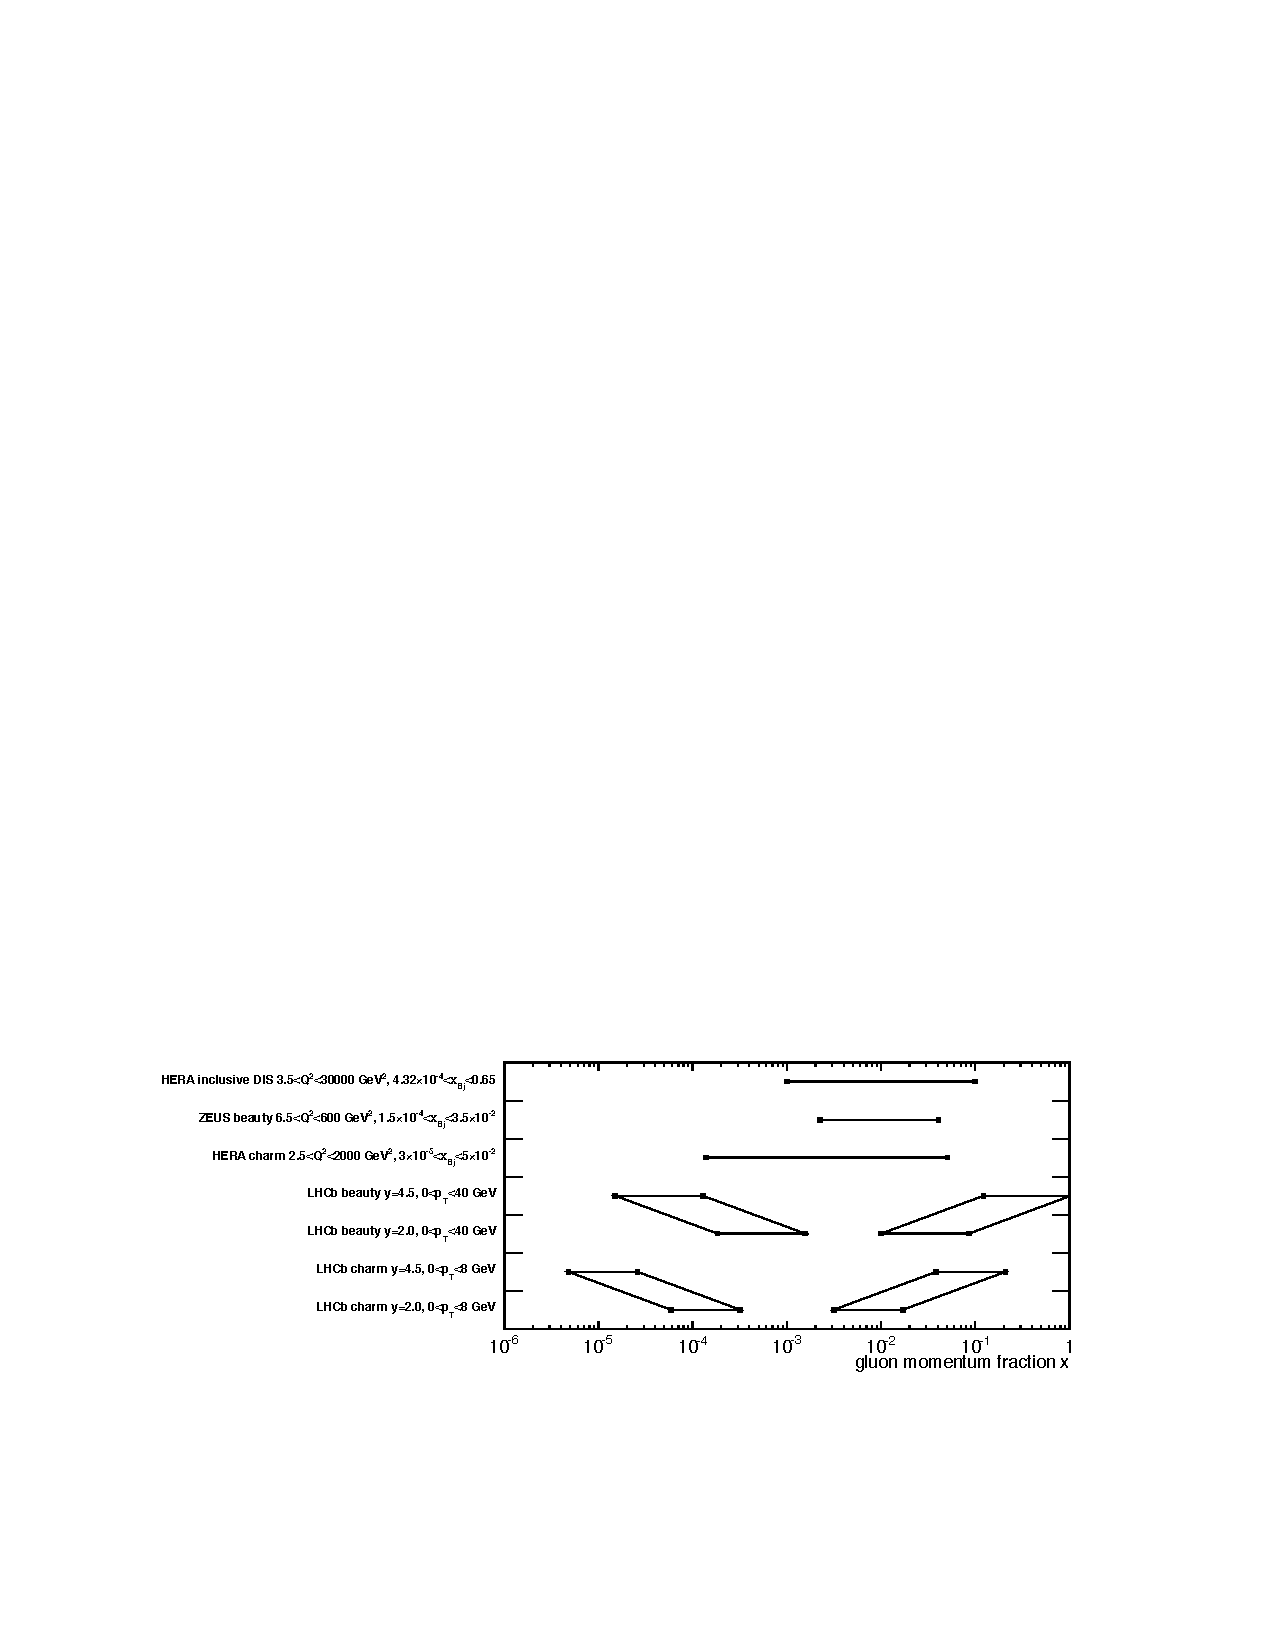
\includegraphics[width=\textwidth]{production/prosa_x_regions}
  \caption{%
    Regions of proton momentum fraction \bjorkenx, on the $x$-axis, probed by 
    different experiments, indicated on the $y$-axis~\cite{Zenaiev:2015rfa}.
  }
  \label{fig:prod:theory:prosa_x_regions}
\end{figure}

\begin{figure}
  \centering
  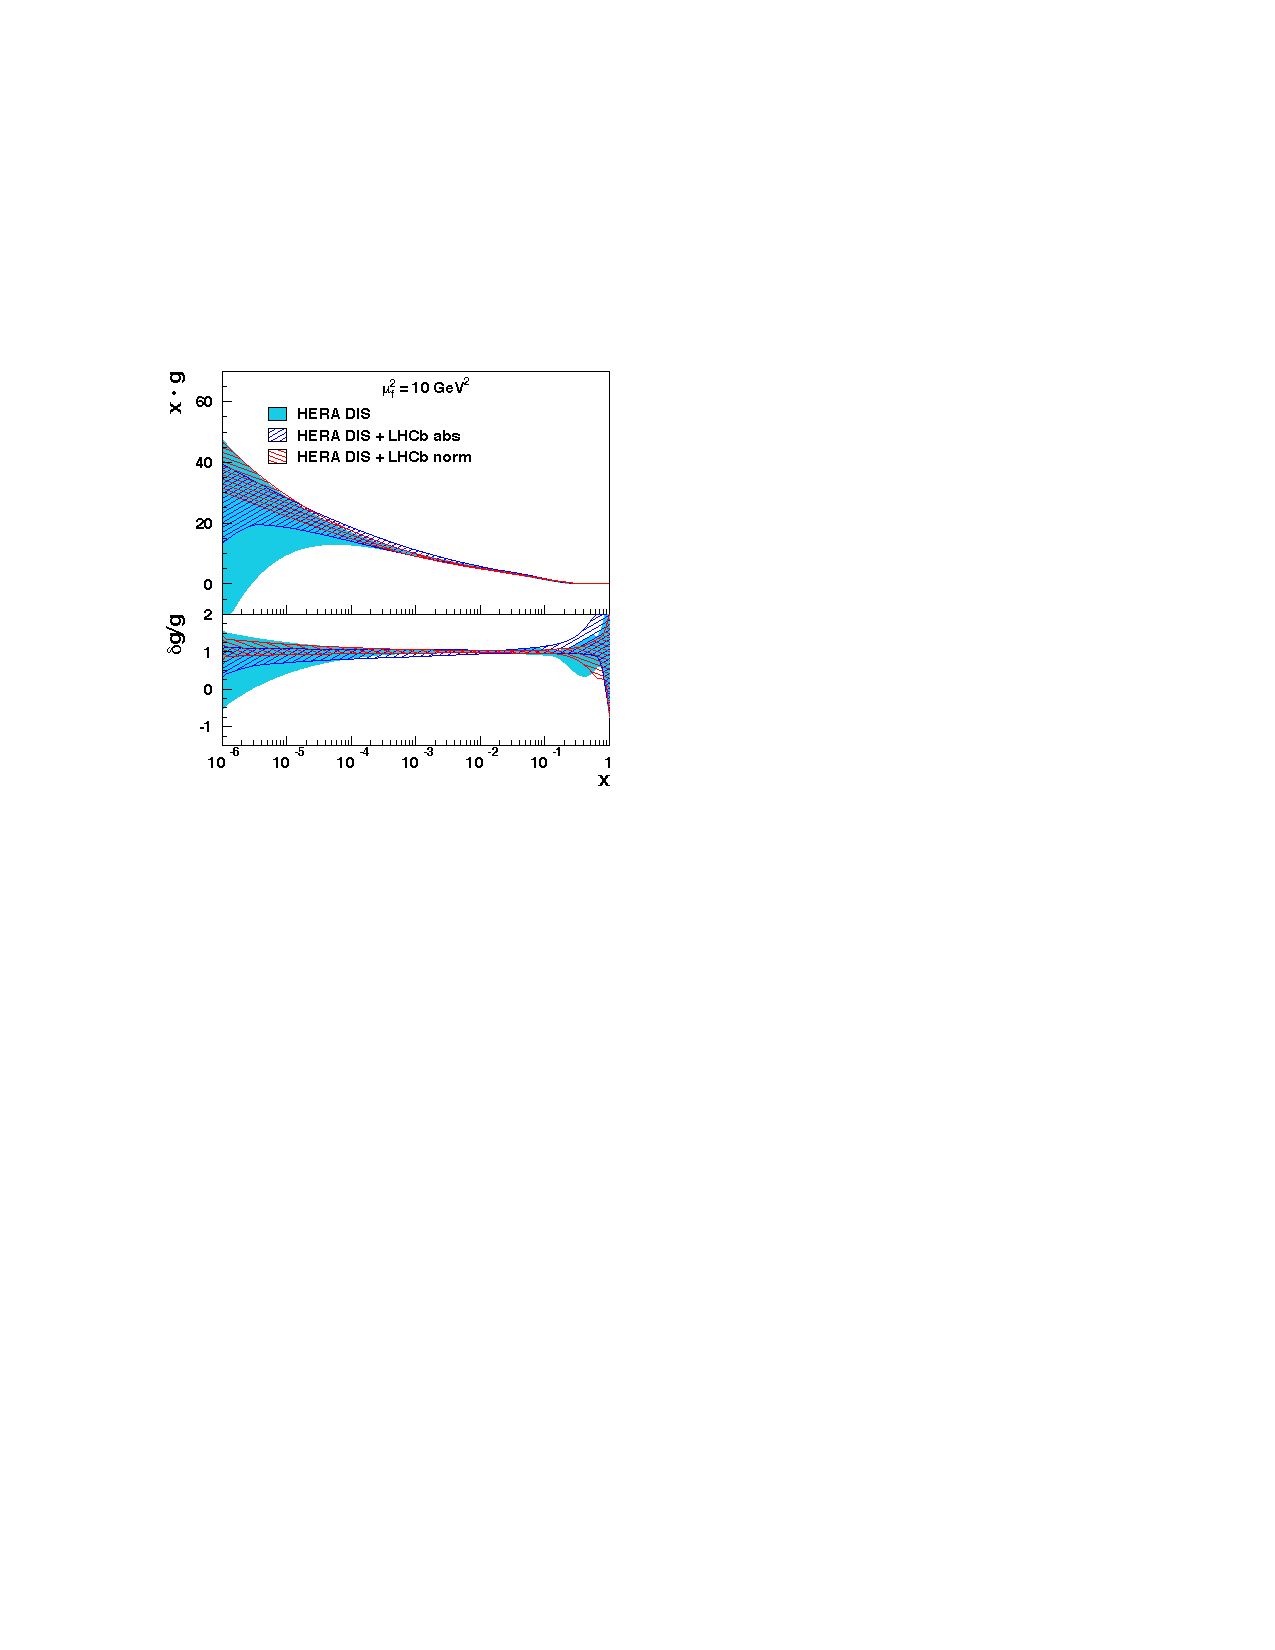
\includegraphics[width=\textwidth]{production/prosa_gluon_pdf_fit}
  \caption{%
    Gluon \acp{QCDPDF} after fitting to experimental 
    data~\cite{Zenaiev:2015rfa}.
    The $x$-axis shows the proton momentum fraction \bjorkenx, the $y$-axis on 
    the top plot shows the gluon \ac{QCDPDF} density, and the $y$-axis on the 
    bottom bottom shows the relative uncertainty on the model.
    The solid band shows the fit when only using the \hera\ measurements as 
    inputs, whilst the hatced bands show the fit when using both the \hera\ and 
    \sqrtseq{7}\ \lhcb\ measurements.
  }
  \label{fig:prod:theory:prosa_gluon_pdf_fit}
\end{figure}

\section{Atmospheric neutrino fluxes}
\label{chap:prod:theory:neutrinos}

The constraints imposed on the proton \acp{QCDPDF} are also useful in 
atmospheric neutrino experiments.
The \icecube\ collaboration aims to measure highly energetic neutrinos of 
astrophysical origin with energies up to the \si{\peta\eV} scale, using the 
IceCube Neutrino Observatory~\cite{Achterberg:2006md}.
This is done to shed light on the mystery of ultra-high-energy cosmic rays 
(protons) whose source is unknown but should also produce similarly energetic
neutrinos.
The so-called conventional neutrino flux constitutes one of the backgrounds for 
astrophysical neutrino experiments.
This is made by cosmic rays interacting in the atmosphere and producing pions 
and kaons, which then decay to final states containing neutrinos.
However, for the high energies the \icecube\ detector is sensitive to, 
beginning at around \SI{100}{\GeV}, this background is suppressed.
The long lifetime of the mesons increases the probability they will interact 
with the atmosphere in flight, losing energy through hadronic interactions, 
hence reducing the energy spectrum of the resulting neutrinos.
However, an additional background comes from the production of charm hadrons in 
the atmosphere, which, with their comparatively short lifetimes, lose very 
little energy in flight, and so the neutrino spectrum from charm decays is very 
similar to the cosmic ray energy spectrum.
The neutrinos produced in the charm decays can interact with the detector in a 
similar manner to the signal and exhibit a similar energy spectrum.
It is then of key importance that the amount of expected background from these 
decays is known, else neutrinos from charm decays may be misinterpreted as 
neutrinos from astrophysical sources.
This contamination can be estimated by predicting the proton-proton 
cross-sections (between the cosmic ray and the nuclei in the atmosphere).

Colliding equal-energy proton-proton beams at a centre-of-mass energy of 
\SI{13}{\TeV} is equivalent to directing a proton beam of energy 
\SI{100}{\peta\eV} into a fixed target, as $\sqrts \approx 
\sqrt{2E_{\Pproton}m_{\Pproton}}$, where $E_{\Pproton}$ is the energy of the 
proton beam and $m_{\Pproton}$ is the proton mass.
Hence, measuring charm cross-sections at \sqrtseq{13}\ at the \ac{LHC} can 
provide constraints on the expected rate of charm production in the atmosphere 
produced by extremely high-energy cosmic rays.
Indeed, the measurements made by \lhcb\ at \sqrtseq{7}\ have already been used 
to that effect, and additional measurements at \SI{13}{\TeV} can help 
further~\cite{Gauld:2015yia,Bhattacharya:2015jpa}.

\section{Cross-section comparisons with theory}
\label{chap:prod:theory:comparisons}

A useful check of \acp{QCDPDF} constrained with past experimental data is to 
compute cross-section predictions using them, for comparison with new 
experimental results.
This was done in the previous \lhcb\ open charm cross-section analysis, shown 
in \cref{fig:prod:theory:comparisons:7tev}, where at low \pT\ the data 
generally lie above the theory prediction.
Additional measurements can help in the understanding of these discrepancies.

For the analysis presented in this \namecref{chap:prod}, a measurement of charm 
production at \sqrtseq{13}, three theory groups have provided predictions for 
the double differential cross-sections.
Each set of predictions is computed at next-to-leading order in the strong 
coupling constant \alphas\ (that is, up to the first power of $\alphas$), and 
includes uncertainties from: the factorisation scale dependence, which is the 
scale \pdfqsquared\ at which the perturbative expansion was made; and the 
renormalisation scale, which is the scale at which the expansion is 
renormalised to remove ultraviolet divergences.
These affect both the evaluation of the partonic cross-sections and the 
evolution of the \ac{QCDPDF} sets with the \ac{DGLAP} equations.

The \nnpdfl\ predictions~\cite{Gauld:2015yia} use a \ac{QCDPDF} set that 
includes the constraints from the \sqrtseq{7}\ \lhcb\ 
measurement~\cite{LHCb-PAPER-2012-041}, and are provided for all \pTy\ bins for 
\PDz and \PDp mesons.
The \ac{GMVFNS} predictions~\cite{Kniehl:2012ti} are provided for $\pT > 
\SI{3}{\GeVc}$ for all mesons under study, and use the CT10 \ac{QCDPDF} set.
These predictions include a factor to account for the \cToHc\ transition 
probability, obtained by convolving the \decay{\ccbar}{\PHc} cross-sections 
with the appropriate fragmentation functions.
Finally, \ac{FONLL} predicitions~\cite{Cacciari:2015fta} using the \nnpdf\ 
\ac{QCDPDF} sets are provided for for the full \pTy\ phase space for \PDz, 
\PDp, and \PDstarp mesons.
The \fonll\ predictions assume a unit \cToHc\ transition probability, and so 
are multiplied by the fragmentation fractions in 
\cref{tab:prod:introduction:fragmentation_fractions} for comparison with the 
measurements.
The comparison of these predictions with the data will be given in 
\cref{chap:prod:results}.

\begin{figure}
  \centering
  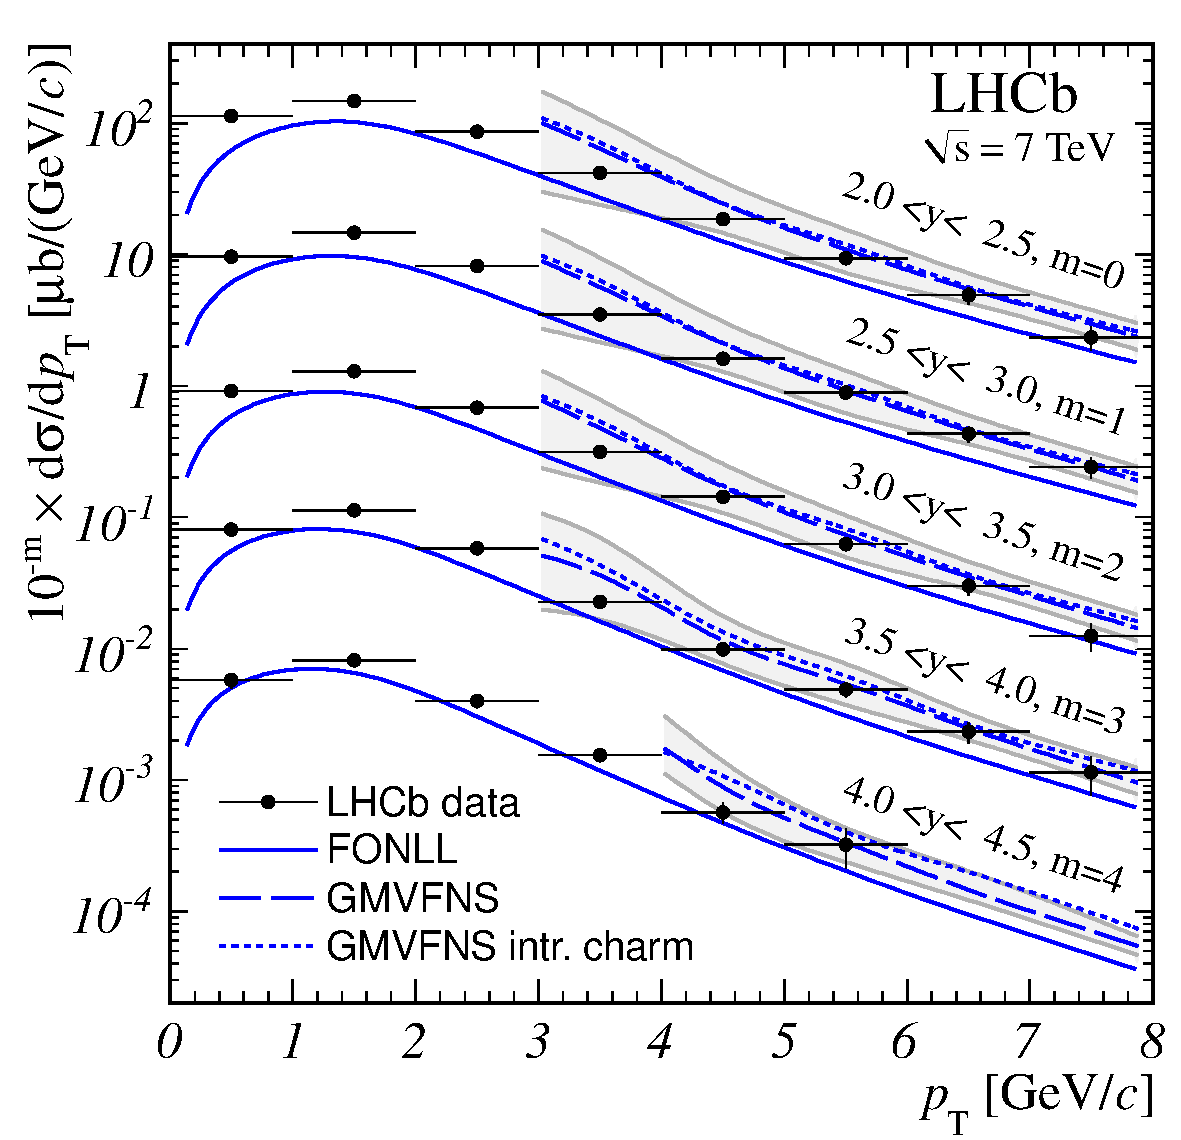
\includegraphics[width=\textwidth]{production/lhcb_dz_xsec_7tev}
  \caption{%
    Prompt \PDzero production rates, measured using the \lhcb\ detector with 
    proton-proton data taken at \sqrtseq{7}~\cite{LHCb-PAPER-2012-041}, in 
    \pTy\ bins.
    The $x$-axis shows the \pT\ of the \PDzero, and the measurements are offset 
    by a multiplicative factor based on the rapidity bin.
  }
  \label{fig:prod:theory:comparisons:7tev}
\end{figure}


\cleardoublepage

\part{%
  \texorpdfstring{\CP\ }{CP} violation in
  \texorpdfstring{%
    \LcTophh
  }{%
    Lambdac+ to ph+h-
  }
  decays
}

\chapter{Introduction}
\label{chap:cpv:introduction}

In 2011, the \lhcb\ collaboration announced the first evidence of \CP\ 
violation in charm decays, claiming a deviation from the \CP\ symmetry 
hypothesis at the
\SI{3.5}{\sigma} level~\cite{Aaij:2011in}.
The measurement was of the difference between the rates of direct \CP\ 
violation in two \ac{SCS} decays of the \PDzero meson, $\decay{\PDzero}{\KmKp}$ 
and \pimpip.

The rate of direct \CP\ violation in the decay of any particle $P$ to a final 
state $f$ is parameterised as
\begin{equation}
  \ACP(\decay{P}{f}) = \frac{%
    \Gamma(\decay{P}{f}) - \Gamma(\decay{\bar{P}}{\bar{f}})
  }{%
    \Gamma(\decay{P}{f}) + \Gamma(\decay{\bar{P}}{\bar{f}})
  }.
  \label{eqn:cpv:introduction:acp}
\end{equation}
For \decay{\PDzero}{\hmhp} decays, this is expected to be of the order of 
\num{e-3} in the \ac{SM}~\cite{Grossman:2006jg}, and as such is sensitive to 
contributions from physics \acl{BSM}.
% TODO should make sure I know what this actually is
Using arguments of $U$-spin symmetry between the \KmKp\ and \pimpip\ final 
states, the sign of $\ACP(\KmKp)$ is predicted to be opposite that of 
$\ACP(\pimpip)$~\cite{Grossman:2006jg}, and so the difference between the two 
is particular sensitive to direct \CP\ violation
\begin{equation}
  \dACP = \ACP(\pKK) - \ACP(\ppipi).
  \label{eqn:cpv:introduction:dacp_pure}
\end{equation}
It was the value of \dACP\ that was measured to deviate significantly from 
zero.

The observation generated much interest in the theory 
community~\cite{Lenz:2013pwa}, creating a push for a better mathematical 
understanding of \CP\ violation in charm decays.
However, subsequent measurements of \dACP, made using larger data samples and 
using \PDzero mesons from \PB\ decays, did not confirm the initial 
evidence~\cite{Aaij:2014gsa,Aaij:2016cfh}, and the current world average is 
consistent with the hypothesis of no direct \CP\ violation in \PDzero 
decays~\cite{Amhis:2014hma}, being\footnotemark
\begin{equation}
  \dACP = \SI{-0.252 \pm 0.104}{\percent}.
  \label{eqn:cpv:introduction:dacp_world_average}
\end{equation}

\footnotetext{%
  The world average is not strictly of \dACP, but of 
  $\Delta{a}_{\CP}^{\text{dir}}$, which includes effects in \emph{indirect} 
  \CP\ violation, which arise to the possibility of \CP\ violation in 
  \PDzero-\APDzero mixing~\cite{Gersabeck:2011xj}.
}

Charm baryons, the lightest of which is the \PLambdac~($\Pup\Pdown\Pcharm)$, 
are an additional system in which to search for \CP\ violation.
The first evidence for \CP\ violation in baryon decays was found only 
recently~\cite{Aaij:2016cla}, using the decays of the lightest beauty baryon, 
the \PLambdab~($\Pup\Pdown\Pbottom$).
An analogous measurement of \dACP\ using \PLambdac\ decays, to that made with 
\PDzero decays, is searching for direct \CP\ violation in the decays \LcTopKK\ 
and \LcToppipi.
The dynamics of these \ac{SCS} decays, which can only be fully parameterised by 
a five-dimensional phase space~\cite{Aitala:1999uq}, are currently poorly 
understood~\cite{Bigi:2012ev,PDG2014}, and so any experimental input can be 
useful to guide and constrain the theory.
The previous generation of heavy flavour collider experiments, such as \belle\ 
and \babar, collected small samples of \PLambdac~\cite{Seuster:2005tr}, whereas 
the large charm cross-section at \lhcb\ enables \CP\ violations measurements at 
the percent level or lower.

The large sample of \PB decays collected by \lhcb\ can also be used to study 
\CP\ violation in \PLambdac\ decays.
The \PLambdab\ has a lifetime around seven times greater than that of the 
\PLambdac, and can be exploited to provide efficient background rejection.
The semileptonic decay chain \LbToLcmuX\ enables the usage of the \lhcb\ muon 
triggers, described in \cref{chap:intro:lhcb:trigger}, requiring a single, high 
\pT\ muon whose trajectory is significantly displaced from the \ac{PV}.
Using measurements of the \LbToLcmuX\ and \LcTophh\ branching 
fractions~\cite{PDG2014,Ablikim:2016tze}, and measurements of the \PLambdab\ 
cross-sections in \pp\ collisions~\cite{Aaij:2015fea}, and assuming a total 
reconstruction and selection efficiency of around \SI{1}{\percent}, \lhcb\ 
should have collected of the order of \num{e4} \ppipi\ decays and \num{e3} \pKK 
decays during \runone.
The statistical uncertainty on a measurement of \dACP\ will then be dominated 
by the \pKK\ sample size, having a precision on the order of 
\SI{0.1}{\percent}.

This analysis measures \dACP\ using \LcTopKK\ and \LcToppipi decays, 
reconstructed in association with a high \pT\ muon assumed to originate from 
the decay of a \PLambdab.
The data used was collected with the \lhcb\ detector in 2011 and 2012, 
corresponding to an integrated luminosity of \SI{3}{\per\femto\barn}.
An overview of the analysis will be given in the remainder of this 
\namecref{chap:cpv:introduction}.

\section{Analysis overview}
\label{chap:cpv:introduction:overview}

Rather than measuring the relative difference of decay rates in 
\cref{eqn:cpv:introduction:acp}, it is simpler to measure the asymmetry in the 
observed yields $N$
\begin{equation}
  \ARaw(f) = \frac{N(f) - N(\bar{f})}{N(f) + N(\bar{f})},
  \label{eqn:cpv:introduction:araw}
\end{equation}
where here, and throughout this \namecref{chap:cpv}, the origin of the final 
state $f$ from a \PLambdac\ decay is implicit.\footnotemark
This is not necessarily equal to the decay asymmetry in 
\cref{eqn:cpv:introduction:acp} as it may contain contributions from associated 
production and detection asymmetries.
The complete formalism and experimental treatment of this will be discussed in 
\cref{chap:cpv:theory}.

\footnotetext{%
  It is assumed that charge is conserved, so a final state $\bar{f}$ implies an 
  initial state \APLambdac.
}

Any theoretical computation of \ACP\ or \dACP\ for \LcTophh\ decays requires 
some model for the five-dimensional \phh\ phase space, as it may be that the 
strength of \CP\ violation varies across it.
The selection and reconstruction of the \PLambdac\ candidates may sculpt this 
distribution, and so the experimental efficiency as a function of the phase 
space must be computed.
The phase space definition is given \cref{chap:cpv:theory:phsp}.

After correcting for any possible background asymmetries with a weighting 
procedure, and for the phase space efficiencies computed using simulated data, 
the \PLambdac\ and \APLambdac\ yields are measured simultaneously for each mode 
with \chisq\ fits.
The fits are performed in such a way that the true value of \ARaw\ is hidden to 
avoid experimental bias, and as such the fits are said to be `blinded'.

The description of the data by the fits, any remaining background asymmetries, 
and \PLambdac\ decays originating from sources other than \PLambdab\ decays are 
considered in the context of systematic uncertainties.
Studies are performed, and deviations from the nominal, measured value of 
\dACP\ that cannot be corrected for will be assigned as systematic 
uncertainties on the measurement.

\subsection{Document structure}
\label{chap:cpv:introduction:overview:structure}

The exact contributions of the various production and detection asymmetries to 
\ARaw will be derived and enumerated in \cref{chap:cpv:theory}.
The parameterisation of the five-dimensional phase space will also be given, 
which is used when constructing the phase space efficiency model.
The collision data and simulated \ac{MC} data used in the analysis is described 
in \cref{chap:cpv:data}, and the reconstruction and selection of the real data 
will be presented in \cref{chap:cpv:selection}.
The extraction of the signal yields and of the kinematic distributions of the 
signal from the fully selected data is presented in 
\cref{chap:cpv:prelim_fits}, and then those signal distributions are equalised 
between the two \PLambdac\ decay modes using \ac{MVA} techniques discussed in 
\cref{chap:cpv:kinematic_weighting}.
The resulting kinematic weights are combined with reconstruction and selection 
efficiencies computed as a function of \phh\ phase space, whose method of 
computation is shown is \cref{chap:cpv:phsp}, after which the combined weights 
enter the blinded \chisq\ fits that are used to measure \ARaw, described in 
\cref{chap:cpv:araw}.
The combination of $\ARaw(\pKK)$ and $\ARaw(\ppipi)$ to measure \dACP\ is in 
\cref{chap:cpv:results}.
Methods for and the results of various systematic studies are given in 
\cref{chap:cpv:syst}.
Finally, \cref{chap:cpv:summary} gives the combination of the measurements of 
\dACP\ and the systematic studies, and concludes with a brief discussion on 
future prospects of \CP\ violation measurements at \lhcb.


\chapter{Formalism}
\label{chap:cpv:theory}

The measurement of \ARaw, as defined in \cref{eqn:cpv:introduction:araw}, can
be contaminated by production and detection asymmetries.
By reconstructing \LcTopKK\ and \LcToppipi\ decays from
\decay{\PLambdab}{\PLambdac\Pmuon X}\ decays, \ARaw\ can include the effects of
the \PLambdab/\APLambdab\ production asymmetry, the \Pmuon/\APmuon detection
asymmetry, and the detection asymmetry of the \PLambdac\ final state
$f$/$\bar{f}$.

The \PLambdab\ production asymmetry is predicted to be non-zero due to the \pp\
collision environment~\cite{PhysRevD.90.014023}, and indeed \lhcb\ has found
evidence of such an asymmetry as a function of \PLambdab\
rapidity~\cite{Aaij:2015fea}.
The two detection asymmetries are also expected to be non-zero, due to the
known differences between the hadron/anti-hadron and muon/anti-muon
cross-sections with matter~\cite{PDG2014}.
The final state detection asymmetry can be broken down into two terms: one due
to the detection asymmetry of the proton; and another due to the detection
asymmetry of the \KmKp pair and the \pimpip\ pair.
If the meson kinematics are equal within a given mode, for example if the
\PKminus kinematics are identical to those of the \PKplus\ in the \pKK\ data,
then the final state asymmetry reduces to the proton detection asymmetry.

Both the \PLambdab\ production and the muon detection asymmetries should be
independent of the \PLambdac\ final state, given the same \PLambdac\
kinematics.
Different acceptance efficiencies between \pKK\ and \ppipi\ can create unequal
\PLambdac\ kinematics, but the kinematics can be weighted to equalise them
between the modes.

It will now be shown how the background asymmetries entering \ARaw\ can be
removed in the difference \dACP\@.
The number of reconstructed \LcTof\ decays can be expressed as the product of
several effective probabilities
\begin{equation}
  N(f) = \prob(\PLambdab)\cdot
         \Gamma(\LbToLcmuX)\cdot
         \Gamma(\LcTof)\cdot
         \eff(\Pmuon)\cdot
         \eff(f),
  \label{eqn:cpv:theory:yield}
\end{equation}
where $\prob(\PLambdab)$ is the probability of producing a $\PLambdab$ baryon
given a \pp\ collision, and $\eff(\Pmuon)$ and $\eff(f)$ are the muon and
$\PLambdac$ final-state detection efficiencies.
A similar expression exists for $N(\bar{f})$, where are particles are replaced
by their charge conjugates.
It is assumed that the \LbToLcmuX\ decay is \CP-symmetric, but that all other
factors may not be, for example $\eff(\Pmuon) \neq \eff(\APmuon)$.

To express \ARaw\ in terms of its component asymmetries, the notation of a
general asymmetry parameter $X$ is defined, which describes the asymmetry
between two quantities $x$ and $\bar{x}$
\begin{equation}
  X = \frac{x - \bar{x}}{x + \bar{x}}.
  \label{eqn:cpv:theory:generic_asym}
\end{equation}
This can be rearranged as
\begin{align}
  x &= \frac{1}{2}(x + \bar{x})(1 + X),\ \text{and}\label{eqn:cpv:theory:asym_form_one}\\
  \bar{x} &= \frac{1}{2}(x + \bar{x})(1 - X).\label{eqn:cpv:theory:asym_form_two}
\end{align}
An asymmetry parameter like that in \cref{eqn:cpv:theory:generic_asym} can be defined for each of the relevant terms in
\cref{eqn:cpv:theory:yield}
\begin{align*}
  \APLb(f) &= \frac{%
    \prob(\PLambdab) - \prob(\APLambdab)
  }{%
    \prob(\PLambdab) + \prob(\APLambdab)
  },\\
  \ADmu(f) &= \frac{%
    \eff(\Pmuon) - \eff(\APmuon)
  }{%
    \eff(\Pmuon) + \eff(\APmuon)
  },\ \text{and}\\
  \ADf(f)  &= \frac{%
    \eff(f) - \eff(\bar{f})
  }{%
    \eff(f) + \eff(\bar{f})
  },
\end{align*}
and the asymmetry in $\Gamma(\LcTof)$ is \ACP\ as in
\cref{eqn:cpv:introduction:acp}.
Each parameter is, at least implicitly, dependent on the detected \PLambdac\
final state, as each parameter can vary in quantities that may also vary
between \PLambdac\ decay modes.
Substituting in Equation~\ref{eqn:cpv:theory:yield} to
Equation~\ref{eqn:cpv:introduction:araw}
\begin{equation*}
  \ARaw(f) = \frac{%
    \prob(\PLambdab)\Gamma(f)\eff(\Pmuon)\eff(f) -
    \prob(\APLambdab)\Gamma(\bar{f})\eff(\APmuon)\eff(\bar{f})
  }{%
    \prob(\PLambdab)\Gamma(f)\eff(\Pmuon)\eff(f) +
    \prob(\APLambdab)\Gamma(\bar{f})\eff(\APmuon)\eff(\bar{f})
  },
\end{equation*}
and then substituting each quantity for its equivalent form as in
\cref{eqn:cpv:theory:asym_form_one,eqn:cpv:theory:asym_form_two}, all factors
of $\sfrac{1}{2}$ and all factors of the form $(x - \bar{x})$ cancel, leaving
\begin{equation}
  \ARaw(f) = \frac{Y}{Z}.
\end{equation}
where (dropping the final state parameter temporarily for compactness)
\begin{align}
  Y = \APLb\ADmu\ADf &+ \APLb\ADmu\ACP + \APLb\ADf\ACP + \ADmu\ADf\ACP \nonumber\\
                     &+ \APLb +  \ADmu + \ADf + \ACP,
\end{align}
and
\begin{align}
  Z = 1 &+ \APLb\ADmu + \APLb\ADf + \APLb\ACP + \ADmu\ADf + \ADmu\ACP \nonumber\\
        &+ \ADf\ACP + \APLb\ADmu\ADf\ACP.
\end{align}
Assuming that the individual asymmetries are small, of the order of
\SI{1}{\percent}, the product of two or more asymmetries is negligible with
respect to the leading order, and so
\begin{equation}
  \ARaw(f) \approx \ACP(f) + \APLb(f) + \ADmu(f) + \ADf(f).
  \label{eqn:cpv:theory:araw_approx}
\end{equation}
By assuming that these background asymmetries are mode-independent, that is to
say $\AD(f) = \AD(g)$ and $\AP(f) = \AP(g)$, the difference between \ARaw\ for
the \pKK\ and \ppipi\ will only have contributions from \ACP
\begin{align}
  \dACP &= \ARaw(\pKK) - \ARaw(\ppipi),\label{eqn:cpv:theory:dacp}\\
        &\approx \ACP(\pKK) - \ACP(\ppipi)\nonumber.
\end{align}

The assumption that the production and detection asymmetries in
\cref{eqn:cpv:theory:araw_approx} are mode independent is not true in general.
This can been seen by first making a weaker assumption that the background
asymmetries are dependent only on the kinematics of the representative
particles.
Different final states will in general have different acceptance,
reconstruction and selection efficiencies as a function of \PLambdac\
kinematics.
The kinematics of the \PLambdac\ are correlated to those of the muon and the
\PLambdab, and so two samples with different \PLambdac\ kinematics will likely
also have different \PLambdab\ and muon kinematics.
Hence, there can still be net production and detection asymmetries in \dACP\@.

The assumption that the background asymmetries depend only on particle
kinematics is not unreasonable.
The production asymmetry, for example, is a difference in cross-sections, which
are usually parameterised by the kinematics of the produced particle (\pT\ and
either \Eta\ or rapidity).
Similarly, a detection asymmetry describes the differences of material
interactions between matter and antimatter, and these are dependent on the
momentum of the particle in question and, assuming a non-uniform material
distribution, its flight path.

As it is not given that the \PLambdac\ kinematics are the same between
\LcTopKK\ and \LcToppipi\ decays in the data, the data can be weighted to
equalise the \PLambdac\ kinematics.
The background asymmetries \AP\ and \ADmu\ will then cancel in the difference
\dACP\@.
The proton kinematics will not necessarily agree after such a weighting, as the
energy release in the \pKK\ and \ppipi\ decays is different.
These considerations govern the analysis strategy: measure the number of
\PLambdac\ candidates in the \pKK\ and \ppipi\ samples after weighting them
such that the \PLambdac\ kinematics look alike, such that the \PLambdab\ and
\Pmuon kinematics also agree.
Additional weighting may be required to equalise the proton kinematics.

\section{Decay phase space}
\label{chap:cpv:theory:phsp}

The phase space of a decay is the set of variables which fully parameterises
all possible dynamics.
Although a three-body decay requires 12 parameters to describe the kinematics,
under the assumptions of four-momentum conservation and that the masses of the
three decay products are known, the number of free parameters is only five.
When all particles involved have zero spin, the distribution of the momenta of
the decay products is isotropic, such that there are only 2 degrees of freedom.
These are usually taken to be two child-pair squared masses, which can be
visualised as a Dalitz plot.
In the case of \LcTophh, the spin \sfrac{1}{2} of the proton means that the
three-body system is no longer rotationally symmetric, and the full five
degrees of freedom are required to describe the phase space.

For a meaningful comparison of the measurement of \dACP\ with theoretical
predictions, which are not presently available, the efficiency of the
\PLambdac\ selection across the five-dimensional phase space must be known.
The definition of ``selection'' includes the effects of the \lhcb\ acceptance
and the trigger, stripping, and offline requirements.
The efficiency model can either be provided to theorists so that they can apply
the same efficiencies to their phase space models, or it can be used to correct
the data before the \dACP\ measurement is made.

The five dimensions of the phase space are defined here in a similar way to the
\LcTopKpi\ amplitude analysis performed by the \esno\
collaboration~\cite{Aitala:1999uq}.
This defines two child-pair squared masses, of the proton and
oppositely-charged child \msqphm\ and of the two opposite-sign pseudo-scalars
\msqhh, and three decay angles.
The child-pair squared masses are invariant under Lorentz transformations, but
the decay angles are not and so a definition of the frame in which they are
computed is required.

The \esno\ analysis defines a coordinate system in the \PLambdac\ rest frame.
The $z$-axis, also called the quantisation axis or polarisation axis \polzlcp,
is perpendicular to the plane of production
\begin{equation}
  z = \polzlcp = \phatbeam \times \phatlcp,
\end{equation}
where \phatbeam\ is the direction of the beam\footnotemark\ and \phatlcp\ is
the direction of the \PLambdac\ measured in the laboratory frame.
\footnotetext{%
  E791 was a fixed-target experiment, colliding a \SI{500}{\GeVc} pion beam
  with metal foils.
}
The $x$-axis of the \PLambdac\ rest frame is \phatlcp.
As the \PLambdac\ candidates in this analysis are not produced directly from
the \pp\ collision but in the decays of \PLambdab\ baryons, here the `beam
direction' is defined as the direction of the \PLambdab\ momentum vector, which
is equal to the direction vector pointing from the \pp\ primary vertex
$v_{\pp}$ to the $\PLambdac\Pmuon$ vertex $v_{\PLambdac\Pmuon}$
\begin{equation}
  \phatbeam = \phatlbz = v_{\PLambdac\Pmuon} - v_{\pp}.
\end{equation}
With this coordinate system and inertial frame, the three decay angles are
defined as:
\begin{enumerate}
  \item The angle \thetap\ between the proton momentum vector and the $z$-axis;
  \item The angle \phip\ between the proton momentum vector and the $x$-axis;
    and
  \item The angle \phihh\ between the plane containing the proton momentum
    vector and the $z$-axis and the plane containing the two pseudo-scalar
    meson momentum vectors.
\end{enumerate}
These definitions are illustrated in \cref{fig:cpv:theory:phsp:angles}

The distributions of the five phase space variables will be presented in
\cref{chap:cpv:phsp}, along with the evaluation of the efficiency as a function
of the position in phase space.

\begin{figure}
  \begin{subfigure}{0.5\textwidth}
    \resizebox{\textwidth}{!}{%
      % Rotation of the axes wrt the viewer
% syntax: \tdplotsetdisplay{\theta_d}{\phi_d}
\tdplotsetmaincoords{70}{110}

% Define proton coordinates
\pgfmathsetmacro{\rp}{.8}
\pgfmathsetmacro{\angthetap}{60}
\pgfmathsetmacro{\angphip}{50}

% Define Kpi coordinates
\pgfmathsetmacro{\rKpi}{.4}
\pgfmathsetmacro{\thetaKpi}{80}
\pgfmathsetmacro{\phiKpi}{340}

% Start a TikZ picture, using the tdplot_main_coords system
% tdplot provides the coordinate transformation
\begin{tikzpicture}[scale=4,tdplot_main_coords]

% Define the origin
\coordinate (O) at (0,0,0);

% Create a point P with coordinates r, theta, and phi
% I think this is similar to \coordinate, but also transform the vector
% in to the rotated coordinate system
\tdplotsetcoord{P}{\rp}{\angthetap}{\angphip}
\tdplotsetcoord{Kpi}{\rKpi}{\thetaKpi}{\phiKpi}

% Draw main coordinate axes
% The anchor key relates to the positioning of the label
% South is towards the bottom of the diagram, east is to the left
\draw[thick,->] (0,0,0) -- (1.0,0,0) node[anchor=north west]{
  $x = \hat{p}_{\PLambdac}$
};
\draw[thick,->] (0,0,0) -- (0,0.5,0) node[anchor=north west]{
  $y$
};
\draw[thick,->] (0,0,0) -- (0,0,0.5) node[anchor=south]{
  $z = \polzlcp = \phatlbz \times \phatlcp$
};

% Draw a vector from origin to point P
% The -stealth' option is the type of arrowhead
\draw[-stealth',color=red] (O) -- (P) node[anchor=west]{\Pproton};
\draw[-stealth',color=red] (O) -- (Kpi) node[anchor=east]{\hmhp};

% Draw projection of vector on to xy plane, and a connecting line
\draw[dashed, color=red] (O) -- (Pxy);
\draw[dashed, color=red] (P) -- (Pxy);

% Draw angle phi of xy projection
% {} arguments are center point, radius, angle-from, angle-to, options, label
% [] arguments are coordinate frame, draw options
\tdplotdrawarc{(O)}{0.25}{0}{\angphip}{anchor=north}{\phip}

%set the rotated coordinate system so the x'-y' plane lies within the
%"theta plane" of the main coordinate system
%syntax: \tdplotsetthetaplanecoords{\phi}
% Rotate the "theta plane" (xz) by phi around z
\tdplotsetthetaplanecoords{\angphip}

% Draw arc in rotated system
\tdplotdrawarc[tdplot_rotated_coords]{(0,0,0)}{0.35}{0}{\angthetap}{anchor=south west}{\thetap}

\end{tikzpicture}

    }
  \end{subfigure}
  \begin{subfigure}{0.5\textwidth}
    \resizebox{\textwidth}{!}{%
      % Rotation of the axes about x-axis, then about z-axis
% We align the x-axis with the negative proton momentum
\tdplotsetmaincoords{0}{0}

% Define proton coordinates
\pgfmathsetmacro{\rp}{0.7}
\pgfmathsetmacro{\angthetap}{90}
\pgfmathsetmacro{\angphip}{180}

% Polarisation axis 'coordinates'
\pgfmathsetmacro{\rpol}{0.7}
\pgfmathsetmacro{\thetapol}{90}
\pgfmathsetmacro{\phipol}{135}

% Define h+h- coordinates
\pgfmathsetmacro{\rKpi}{.4}
\pgfmathsetmacro{\thetaKpi}{80}
\pgfmathsetmacro{\phiKpi}{340}

% Define h+ coordinates
\pgfmathsetmacro{\rhp}{.4}
\pgfmathsetmacro{\thetahp}{90}
\pgfmathsetmacro{\phihp}{-20}

% Define h+ coordinates
\pgfmathsetmacro{\rhm}{.6}
\pgfmathsetmacro{\thetahm}{90}
\pgfmathsetmacro{\phihm}{30}

% Start a TikZ picture, using the tdplot_main_coords system
% tdplot provides the coordinate transformation
\begin{tikzpicture}[scale=4,tdplot_main_coords]

% Define the origin
\coordinate (O) at (0,0,0);

% Create a point P with coordinates r, theta, and phi
% I think this is similar to \coordinate, but also transform the vector
% in to the rotated coordinate system
\tdplotsetcoord{P}{\rp}{\angthetap}{\angphip}
\tdplotsetcoord{Hp}{\rhp}{\thetahp}{\phihp}
\tdplotsetcoord{Hm}{\rhm}{\thetahm}{\phihm}
\tdplotsetcoord{Pol}{\rpol}{\thetapol}{\phipol}
\tdplotsetcoord{Kpi}{\rKpi}{\thetaKpi}{\phiKpi}

% h+h- plane parameters
\pgfmathsetmacro{\hhHeight}{1}
\pgfmathsetmacro{\hhWidth}{0.7}
\pgfmathsetmacro{\hhSkew}{30}
\pgfmathsetmacro{\hhSkewWidth}{tan(\hhSkew)*\hhHeight}
\coordinate (hhOrigin) at ($(-\hhSkewWidth/2,-0.5)$);

% Draw planes before anything else, as fill would cover them
% Proton-z plane
\filldraw[semithick,black,fill=white] ($(P)-(0.1,0.6)$) rectangle (0,0.8);
% h+h- plane
\filldraw[semithick,black,fill=white] (hhOrigin)
  -- ($(hhOrigin)+(\hhSkewWidth, \hhHeight)$)
  -- ($(hhOrigin)+(\hhSkewWidth+\hhWidth,\hhHeight)$)
  -- ($(hhOrigin)+(\hhWidth, 0)$)
  % Close the path
  -- cycle;
% Angle between planes
% \draw[dotted] (hhOrigin) -- ($(hhOrigin)+(0, \hhHeight)$);
\tdplotdrawarc[dotted,very thick]{(O)}{0.5}{90}{
  90-\hhSkew
}{anchor=south west}{\Large$2\pi - \phihh$}

% Draw main coordinate axes
% The anchor key relates to the positioning of the label
% South is towards the bottom of the diagram, east is to the left
% \draw[thick,->] (O) -- (1,0,0) node[anchor=north west]{
%   $x = \hat{p}_{\PLambdac}$
% };
% \draw[thick,->] (O) -- (0,1,0) node[anchor=north west]{
%   $y$
% };

% Proton
\draw[-stealth',color=red] (O) -- (P) node[anchor=south]{\Large\Pproton};
% Polarisation axis
\draw[thick,->] (O) -- (Pol) node[anchor=south]{
  \Large$z = \polzlcp$
};

% h+
\draw[-stealth',color=red] (O) -- (Hp) node[anchor=north]{\Large\Php};
% h-
\draw[-stealth',color=red] (O) -- (Hm) node[anchor=south]{\Large\Phm};

% Draw projection of vector on to xy plane, and a connecting line
% \draw[dashed, color=red] (O) -- (Pxy);
% \draw[dashed, color=red] (P) -- (Pxy);

% Draw angle phi of xy projection
% {} arguments are center point, radius, angle-from, angle-to, options, label
% [] arguments are coordinate frame, draw options
\tdplotdrawarc{(O)}{0.25}{\angphip}{\phipol}{anchor=east}{\Large\thetap}

%set the rotated coordinate system so the x'-y' plane lies within the
%"theta plane" of the main coordinate system
%syntax: \tdplotsetthetaplanecoords{\phi}
% Rotate the "theta plane" (xz) by phi around z
% \tdplotsetthetaplanecoords{\angphip}

% Draw arc in rotated system
% \tdplotdrawarc[tdplot_rotated_coords]{(0,0,0)}{0.35}{0}{\angthetap}{anchor=south 
% west}{$\theta_{p}$}

\end{tikzpicture}

    }
  \end{subfigure}
  \caption{%
    Definition of inertial reference frame axes and \LcTophh\ phase space decay
    angles.
    Adapted from Figure~1 in the \esno\ \LcTopKpi\ amplitude analysis
    paper~\cite{Aitala:1999uq}.
  }
  \label{fig:cpv:theory:phsp:angles}
\end{figure}


\cleardoublepage

\part{Monitoring the \lhcb\ vertex locator detector}

\chapter{Introduction}
\label{chap:moni:introduction}

\lipsum[1-12]


\cleardoublepage

\appendix

\appendixpage*

\chapter{Derivation of complicated equation}
\label{chap:derivation}

\lipsum[1-2].


\backmatter

\chapter{Acronyms}

\begin{acronym}
  \acro{QCD}{quantum chromodynamics}
  \acro{EM}{electromagnetic}
  \acro{EW}{electroweak}
  \acro{SM}{standard model}
  \acro{BSM}{beyond the \acl{SM}}
  \acro{CF}{Cabibbo-favoured}
  \acro{SCS}{singly Cabibbo-suppressed}
  \acro{DCS}{doubly Cabibbo-suppressed}

  \acro{QCDPDF}[PDF]{parton density function}
  \acro{DGLAP}{Dokshitzer-Gribov-Lipatov-Altarelli-Parisi}
  \acro{DIS}{deep inelastic scattering}
  \acro{\fonll}{fixed-order next-to-leading logarithms}
  \acro{\gmvfns}{generalised-mass variable-flavour-numbering scheme}

  \acro{MC}{Monte Carlo}
  \acro{PDF}{probability density function}
  \acro{MVA}{multivariate analysis}
  \acro{BDT}{boosted decision tree}
  \acro{KDE}{kernel density estimate}

  \acro{PV}{primary vertex}
  \acro{IP}{impact parameter}
  \acro{DOCA}{distance of closest approach}
  \acro{DIRA}{direction angle}
  \acro{DLL}{delta-log-likelihood}
  \acro{PID}{particle identification}

  \acro{L0}{level-zero}
  \acro{HLT}{high level trigger}

  \acro{LHC}{Large Hadron Collider}
  \acro{LS1}{\lsone}
  \acro{LHCIP}[IP]{interaction point}
  \acro{GPD}{general purpose detector}

  \acro{VDM}{van der Meer}
  \acro{BGI}{beam-gas imaging}

  \acro{PDG}{Particle Data Group}
\end{acronym}


\bibliographystyle{unsrt}
\renewcommand{\bibname}{References}
\bibliography{bibliography}

\end{document}
